\documentclass[a5paper]{article}
\usepackage[a5paper, top=8mm, bottom=8mm, left=8mm, right=8mm]{geometry}

\usepackage{polyglossia}
\setdefaultlanguage[babelshorthands=true]{russian}

\usepackage{fontspec}
\setmainfont{FreeSerif}
\newfontfamily{\russianfonttt}[Scale=0.7]{DejaVuSansMono}

\usepackage[font=scriptsize]{caption}

\usepackage{amsmath}
\usepackage{amssymb,amsfonts,textcomp}
\usepackage{color}
\usepackage{array}
\usepackage{hhline}
\usepackage{cite}

\usepackage[hang,multiple]{footmisc}
\renewcommand{\footnotelayout}{\raggedright}

\PassOptionsToPackage{hyphens}{url}\usepackage[xetex,linktocpage=true,plainpages=false,pdfpagelabels=false]{hyperref}
\hypersetup{colorlinks=true, linkcolor=blue, citecolor=blue, filecolor=blue, urlcolor=blue, pdftitle=1, pdfauthor=, pdfsubject=, pdfkeywords=}

\usepackage{tabu}

\usepackage{graphicx}
\usepackage{indentfirst}
\usepackage{multirow}
\usepackage{subfig}
\usepackage{footnote}
\usepackage{minted}

\sloppy
\pagestyle{plain}

\title{Событийно-ориентированное программирование}
\author{Юрий Литвинов\\\small{yurii.litvinov@gmail.com}}

\date{29.03.2019г}

\begin{document}

\maketitle
\thispagestyle{empty}

\section{Введение}

В этой лекции речь пойдёт про событийную систему C\# и лямбда-функции. Лямбда-функции, на самом деле, очень полезны и безотносительно событийно-ориентированного программирования, но оказываются очень удобны в качестве обработчиков событий (только использовать их в этом качестве надо очень аккуратно, иначе утечки памяти гарантированы). 

Нужна событийная система прежде всего для разработки программ с пользовательским интерфейсом. В отличие от большинства консольных программ, программы с пользовательским интерфейсом не управляют сами процессом вычисления, а ждут событий извне (например, что пользователь кликнет на кнопку) и реагируют на них. Делается это с помощью системной очереди сообщений, в которую сама операционная система ставит событие, и цикла обработки событий, в котором оконное приложение проверяет очередь сообщений и, если она не пуста, забирает оттуда событие  и обрабатывает его. При этом, как правило, библиотека, на базе которой написано оконное приложение, занимается диспетчеризацией события, то есть находит конкретный элемент управления, которому событие предназначено, и вызывает правильный обработчик события. Дело прикладного программиста --- лишь переопределить обработчики.

Событийное программирование применяется не только для разработки оконных приложений. Вообще, большая часть приложений, работающих в мире, запускается и ждёт наступления какого-либо события --- поступления сетевого запроса, срабатывания датчика, действия пользователя, события от таймера и т.д. Постоянно крутиться в цикле и проверять, не произошло ли событие сейчас, нельзя, потому что непрерывно исполняющийся бесконечный цикл загружает на 100\% ядро процессора, что негативно сказывается на энергопотреблении, шуме от вентилятора и работоспособности остальной системы. Поэтому поток, ожидающий события, блокируется операционной системой до того, как ожидаемое событие не наступит, и системных ресурсов почти не потребляет.

Обработка событий когда-то давно реализовывалась с помощью такого понятия, как callback. Колбэк --- это, по сути, указатель на функцию, которую можно вызвать. Так, например, работал старый WinAPI (программный интерфейс операционной системы Windows) --- если мы хотим ловить в нашей программе событие <<пользователь нажал на кнопку>>, мы создаём функцию, которая будет обрабатывать это событие, берём указатель на неё, и передаём оконной системе, чтобы она связала кнопку и этот указатель. Тогда по нажатию на кнопку по указателю вызовется функция. Это плохо вяжется с ООП, потому что есть виртуальные методы (конкретный адрес, по которому надо передать управление, может быть неизвестен во время компиляции).

Более объектно-ориентированный способ --- когда библиотека определяет в классе ``Кнопка'' абстрактный метод ``РеагироватьНаКлик'', а в пользовательском коде мы наследуемся от кнопки и переопределяем этот метод так, чтобы он делал что-нибудь полезное. Оконная библиотека, когда получила событие, вызывает у кнопки её метод и происходит вызов переопределённого метода у потомка. Этот приём называется ``Inversion of Control'' --- не мы вызываем библиотечный код, а библиотека наш. Используется этот приём, как обычно, не только в оконных приложениях, но и везде, где существенную часть всяких рутинных действий по организации процесса вычисления можно вынести в библиотеку (те же веб-приложения устроены так же).

Ещё более идеологически правильным решением является паттерн <<Наблюдатель>>. Этот паттерн заключается в том, что есть наблюдаемый объект, который может производить некоторые события, и есть наблюдающие за ним объекты, которые хотят получать оповещения об этих событиях. В таком случае, наблюдающие объекты регистрируются в наблюдаемом (обычно просто заносятся в список), и когда в наблюдаемом объекте происходит какое-то событие, наблюдаемый объект бежит по списку наблюдателей, говоря каждому, что произошло событие:

\begin{center}
	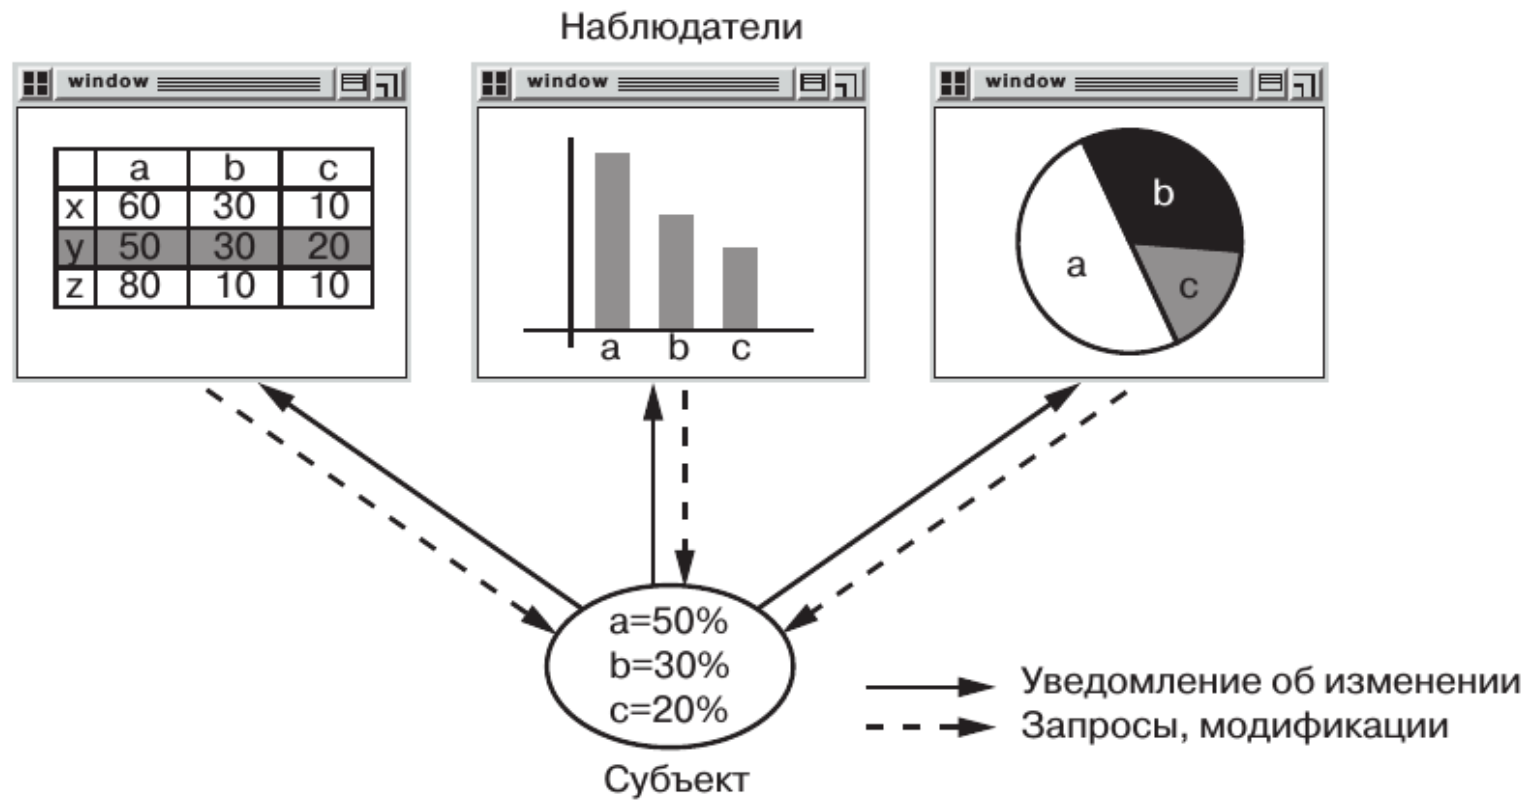
\includegraphics[width=0.7\textwidth]{observerExample.png}
\end{center}

Вот диаграмма классов, которая обобщает изложенное выше:

\begin{center}
	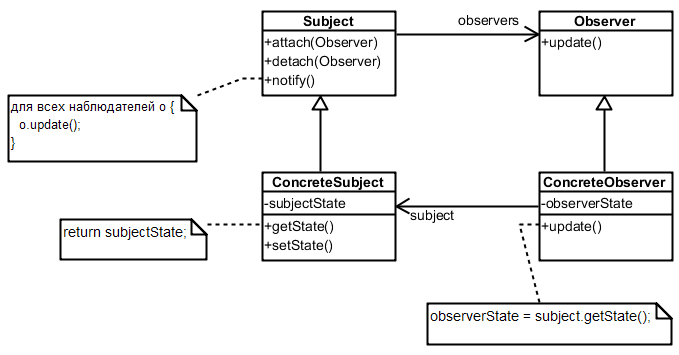
\includegraphics[width=0.7\textwidth]{observer.png}
\end{center}

Subject --- это штука, которая может производить события (например, кнопка). У неё есть методы, позволяющие зарегистрировать наблюдателей (класс Observer), и метод notify(), который бежит по списку зарегистрированных наблюдателей и вызывает их метод, ответственный за обработку события (тут update()). При этом подробности произошедшего либо прямо передаются как параметры в этот метод, либо наблюдатель может спросить у субъекта подробности сам (как тут ConcreteObserver, наследующийся от Observer, может спросить у ConcreteSubject детали через метод getState()).

Собственно, в Java долгое время обработчики событий реализовывались буквально как в этом паттерне. Создавался класс, реализующий интерфейс ActionListener, состоящий из одного метода actionPerformed, где и делается всё, что надо делать по клику на кнопку. Потом с помощью вызова метода кнопки addActionListener объект этого класса регистрировался в кнопке. Потом пользователь нажимал на кнопку, кнопка обходила список объектов типа ActionListener, вызывая их методы actionPerformed. Чтобы это было удобно (не приходилось долго и мучительно передавать состояние в объект-обработчик), в Java даже сделали весьма странный языковой механизм --- нестатические вложенные классы, которые неявно хранили ссылку на объект объемлющего класса, который их создал. Кроме того, в Java есть <<анонимные классы>>, или объектные выражения, которые могут реализовывать интерфейс прямо на месте, при вызове addActionListener. Такой объект, объявленный локально в методе, имел ещё и доступ к локальным переменным метода (то есть реализовывалось честное замыкание), так что до лямбда-функций оставался один шаг, который и был сделан в 2014 году в Java 8. В C\# всё появилось гораздо раньше.

\section{Делегаты}

На самом деле, работа с событиями достаточно важна, чтобы в C\# появилась довольно мощная языковая поддержка для паттерна <<Наблюдатель>> (как ни странно, в отличие от Java, где всё ограничилось анонимными классами и лямбда-функциями). Но появилась эта поддержка не сразу, язык эволюционировал, и довольно уродливый синтаксис первых версий языка постепенно заменился на довольно удобный синтаксис, который используется сейчас. Но поскольку эволюция шла в направлении повышения уровня абстракции, и каждый следующий вид синтаксиса на самом деле базируется на предыдущих, то имеет смысл повторить этот путь, благо в коде и в различной документации часто можно наткнуться на термины типа <<Делегат>>. Собственно, с делегатов и начнём.

Делегат в .NET --- это объект, который по сути является ссылкой на некоторый метод. Тут важно, что делегат --- это объект, он довольно многое знает о том методе, на который ссылается: его параметры (с типами), тип возвращаемого значения, адрес того метода, который надо вызвать, переменные, попавшие в замыкание делегата (но об этом попозже). В делегате можно сохранить ссылку на метод, передать куда-нибудь делегат, а потом вызвать делегат, при этом вызовется тот метод, который там лежит. 

Делается это так. Сначала надо объявить тип делегата:

\begin{minted}{csharp}
public delegate void Feedback(int value);
\end{minted}

delegate --- ключевое слово, Feedback --- имя типа делегата. Такой делегат может хранить в себе ссылку на любой метод, принимающий один \mintinline{csharp}|int|-овый параметр и ничего не возвращающий. На самом деле, Feedback --- это автоматически генерируемый компилятором класс, наследуемый от библиотечного класса System.MulticastDelegate, который в свою очередь наследуется от System.Delegate, у него есть всякие методы, самый интересный из которых --- генерируемый компилятором метод Invoke(...), вызов метода, на который делегат ссылается. Invoke имеет те же параметры, что и сам делегат, в данном случае, \mintinline{csharp}|int|, и возвращает то, что возвращает делегат, в данном случае --- ничего. 

Ещё есть методы BeginInvoke(...) и EndInvoke(), позволяющие вызвать делегат асинхронно. Это довольно часто использовавшийся раньше в стандартной библиотеке паттерн обеспечения асинхронных вызовов, Begin... инициирует асинхронную операцию, принимая необходимые аргументы и колбэк, и тут же возвращая управление вызывающему. Операция исполняется в параллельном потоке, и когда она заканчивает исполнение, вызывается колбэк (в потоке делегата, не в вызывающем), который может получить доступ к результатам вычислений, выполненных делегатом, с помощью метода EndInvoke.

Интересно, что для вызова делегата можно обойтись и без Invoke, а просто вызвать делегат, как будто это обычная функция:

\begin{minted}{csharp}
public delegate int HashFunction(string str, int hashSize);

private static class HashFunctions
{
    public static int Hash1(string str, int hashSize)
    {
        return str[0] % hashSize;
    }

    public static int Hash2(string str, int hashSize)
    {
        int result = 0;
        foreach (var ch in str)
        {
            result += ch;
        }

        return result % hashSize;
    }
}

static void Main(string[] args)
{
    var h = new HashFunction(HashFunctions.Hash1);
    var result = h("ololo", 10);
}
\end{minted}

Тут вызовется статический метод HashFunctions.Hash1.

\section{Пример: цикл обработки событий}

Делегаты даже в таком виде можно использовать для реализации событийной схемы. Собственно, можно построить модель своей собственной <<оконной системы>> с циклом обработки событий и обработчиками. Она у нас будет очень простая, но вполне подойдёт для примера, который будет постепенно эволюционировать, следуя за появлением языковых особенностей в C\#. Положим, мы пишем компьютерную игру, и хотим, чтобы она реагировала на нажатие стрелочек на клавиатуре. Было бы разумно разделить пользовательский ввод и реакцию на действия пользователя по разным классам, так что нам потребуются классы EventLoop и Game. Псевдокод цикла обработки событий выглядел бы так:

\begin{minted}{csharp}
public class EventLoop
{
    public void Run()
    {
        while (true)
        {
            var key = Console.ReadKey();
            switch (key.Key)
            {
                case ConsoleKey.LeftArrow:
                    // Сделать что-то по нажатию на "влево"
                    break;
                case ConsoleKey.RightArrow:
                    // Сделать что-то по нажатию на "вправо"
                    break;
            }
        }
    }
}

static void Main(string[] args)
{
    var eventLoop = new EventLoop();
    eventLoop.Run();
}
\end{minted}

Попользуем делегаты для того, чтобы задавать нужную нам функциональность как реакцию на события нажатия клавиш:

\begin{minted}{csharp}
public delegate void ArrowHandler();

public class EventLoop
{
    public void Run(ArrowHandler left, ArrowHandler right)
    {
        while (true)
        {
            var key = Console.ReadKey(true);
            switch (key.Key)
            {
                case ConsoleKey.LeftArrow:
                    left();
                    break;
                case ConsoleKey.RightArrow:
                    right();
                    break;
            }
        }
    }
}

public class Game
{
    public void OnLeft()
    {
        Console.WriteLine("Going left");
    }

    public void OnRight()
    {
        Console.WriteLine("Going right");
    }
}

static void Main(string[] args)
{
    var eventLoop = new EventLoop();
    var game = new Game();
    eventLoop.Run(new ArrowHandler(game.OnLeft), new ArrowHandler(game.OnRight));
}
\end{minted}

Обратите внимание, метод Main остаётся очень простым, всё, что он делает --- это связывает цикл обработки событий и игру. Ни игра ничего не знает о цикле обработки событий, ни цикл обработки событий ничего не знает об игре, что даёт нам возможность переиспользовать эти классы в разных других ситуациях.

\section{Комбинирование делегатов}

Паттерн <<Наблюдатель>> прекрасно работает, если за одним объектом хотят наблюдать сразу несколько наблюдателей (они просто добавляются в список, и наблюдаемый объект сообщает о событии им всем). У нас пока что так нельзя, потому что делегаты передаются в конструктор нашего цикла обработки событий. Допустим, мы хотим помимо собственно игры прицепить к циклу обработки событий объект для записи действий пользователя, который бы, например, запоминал, куда ходил пользователь, и отправлял бы данные на сервера тайного мирового правительства. Это можно сделать прямо в Game, но это архитектурно плохо, потому что эта функциональность к Game не относится, и было бы хорошо, если бы Game вообще ничего про это не знала. Делегаты так умеют --- они поддерживают так называемый мультикастинг, то есть рассылку сообщения множеству адресатов. Делегату можно приписать ещё один метод, который он будет вызывать, когда его вызовут, с помощью оператора +=, или статического метода Delegate.Combine. Можно было бы написать вот такой код, который бы позволил зарегистрировать больше одного делегата на одно и то же событие:

\begin{minted}{csharp}
public void Register(SomeDelegateType someDelegate)
{
    if (currentDelegate == null) 
    {
        currentDelegate = someDelegate;
    }
    else
    {
        Delegate.Combine(currentDelegate, someDelegate);
    }
}
\end{minted}

Более понятно должно быть из большого примера:

\begin{minted}{csharp}
public delegate void ArrowHandler();

public class EventLoop
{
    private ArrowHandler leftHandler;
    private ArrowHandler rightHandler;

    public void RegisterLeftHandler(ArrowHandler left)
    {
        leftHandler += left;
    }

    public void RegisterRightHandler(ArrowHandler right)
    {
        rightHandler += right;
    }

    public void Run()
    {
        while (true)
        {
            var key = Console.ReadKey(true);
            switch (key.Key)
            {
                case ConsoleKey.LeftArrow:
                    if (leftHandler != null)
                    {
                        leftHandler();
                    }

                    break;
                case ConsoleKey.RightArrow:
                    if (rightHandler != null)
                    {
                        rightHandler();
                    }

                    break;
            }
        }
    }
}

public class Game
{
    public void OnLeft()
    {
        Console.WriteLine("Going left");
    }

    public void OnRight()
    {
        Console.WriteLine("Going right");
    }
}

public class Logger
{
    private List<string> log = new List<string>();

    public void LeftPressed()
    {
        log.Add("left");
    }

    public void RightPressed()
    {
        log.Add("right");
    }
}

static void Main(string[] args)
{
    var eventLoop = new EventLoop();
    var game = new Game();
    var logger = new Logger();

    eventLoop.RegisterLeftHandler(game.OnLeft);
    eventLoop.RegisterRightHandler(game.OnRight);

    eventLoop.RegisterLeftHandler(logger.LeftPressed);
    eventLoop.RegisterRightHandler(logger.RightPressed);

    eventLoop.Run();
}
\end{minted}

Мы тут ещё пользуемся механизмом, называющимся Method Group Conversion --- явно не создаём объект делегата, передавая в метод, принимающий делегат, прямо метод, на который этот делегат должен указывать. Например, eventLoop.RegisterLeftHandler(game.OnLeft);. Это то же самое, что и создание делегата, только короче. Ещё обратите внимание, что мы проверяем делегат на null перед вызовом --- теперь может так оказаться, что никто не добавит свой обработчик, при этом программа не должна падать.

Можно и отписываться от событий, используя оператор -=, например, можно сделать метод 

\begin{minted}{csharp}
public void UnregisterLeftHandler(ArrowHandler left)
{
    leftHandler -= left;
}
\end{minted}

Делать подобные методы обычно весьма мудро, потому что пока делегат добавлен в какую-нибудь цепочку вызовов, сборщик мусора не может его собрать, а значит, не может собрать и все объекты, на которые делегат ссылается. Случайно не отписанный вовремя делегат может иметь ужасные последствия в плане скорости работы и занимаемой памяти. Представим себе ситуацию, когда, например, при переинициализации рабочей области текстового редактора (например, при открытии документа) мы подписываем делегаты, обрабатывающие события нажатия на клавиши, и случайно забываем отписать те делегаты, что уже были подписаны. Если при этом редактор устроен так, что обработчики только лишь запрашивают состояние рабочей области, обновляют внутреннюю структуру документа и не производят видимых эффектов, то проблему можно будет заметить только через несколько тысяч открытий документов --- редактор станет работать заметно медленнее. Вряд ли такой баг будет замечен при тестировании.

\section{Внутреннее устройство цепочек делегатов}

Чтобы окончательно разобраться, что происходит в делегатах с цепочками, можно посмотреть на то, как примерно выглядит сгенерированный метод Invoke для делегата Feedback, с которого начинался этот рассказ:

\begin{minted}{csharp}
public Int32 Invoke(Int32 value) {
    Int32 result;
    Delegate[] delegateSet = _invocationList as Delegate[];
    if (delegateSet != null) 
    {
        foreach (Feedback d in delegateSet)
        {
            result = d(value);
        }
    } 
    else 
    {
        result = _methodPtr.Invoke(_target, value);
    }

    return result;
}
\end{minted}

Видим, что \_invocationList --- это просто массив длегатов, и если он \mintinline{csharp}|null|, то ничего интересного не происходит --- вызывается метод и возвращается его значение. А вот если он не \mintinline{csharp}|null|, то делегаты последовательно вызываются из массива, при этом <<наше>> значение \_methodPtr даже не используется. Ещё, что важно, если делегатов несколько, то и результатов несколько, так что результатом вызова цепочки станет результат последнего вызыванного делегата. Обычно порядок делегатов в цепочке сложно предсказать --- он соответствует порядку, в котором делегаты подписывались, но объект, посылающий событие, вряд ли может знать, кто и в каком порядке на него подписан. Поэтому использовать цепочки делегатов рекомендуется (очень рекомендуется) только в случае, если они возвращают \mintinline{csharp}|void|, либо возвращаемое значение можно проигнорировать. То же самое с исключениями --- если кто-то из цепочки бросит исключение, оставшиеся делегаты даже не будут вызваны, что не всегда желательно.

В принципе, цепочка делегатов доступна с помощью метода GetInvocationList() у делегата, так что вызов делегатов из цепочки можно сделать и вручную, так:

\begin{minted}{csharp}
Delegate[] arrayOfDelegates = leftHandler.GetInvocationList();
foreach (ArrowHandler handler in arrayOfDelegates) 
{
    try 
    {
        handler.Invoke();
    }
    catch (InvalidOperationException e) 
    {
        Object component = handler.Target;
        Console.WriteLine(
                "Failed to call handler from {1}{2}{0} Error: {3}{0}{0}",
                Environment.NewLine,
                ((component == null) ? "" : component.GetType() + "."),
                handler.GetMethodInfo().Name,
                e.Message);
    }
}
\end{minted}

Тут, если делегат из цепочки бросил исключение, исключение обрабатывается и делегаты из цепочки спокойно вызываются дальше.

\section{Шаблонные типы-делегаты}

Кучу кода из приведённого примера с циклом обработки событий на самом деле можно не писать. Первое, что можно заметить, что обработчик события нажатия на кнопку --- это просто метод, который ничего не принимает и ничего не возвращает, нам не важно, как называется тип делегата, и никакого преимущества от объявления типа ArrowHandler мы не получили. Поэтому в стандартной библиотеке объявлены классы Action и Func, Action представляет собой генерик-делегат, принимающий до 15 каких угодно параметров и ничего не возвращающий. Func представляет делегат, который принимает до 15 параметров любого типа и возвращает значение. Например, вместо ArrowHandler можно было писать просто Action, а вместо делегата из самого начала, 

\begin{minted}{csharp}
public delegate int HashFunction(string str, int hashSize);
\end{minted}

можно было использовать \mintinline{csharp}|Func<string, int, int>|. Два первых параметра-типа --- это аргументы, последний --- тип возвращаемого значения. Func и Action появились в стандартной библиотеке не сразу, поэтому в самой библиотеке нередки объявления типов-делегатов. На самом деле, по словам Джеффри Рихтера, ситуация в стандартной библиотеке была примерно такой:

\begin{minted}{csharp}
public delegate void TryCode(Object userData);
public delegate void WaitCallback(Object state);
public delegate void TimerCallback(Object state);
public delegate void ContextCallback(Object state);
public delegate void SendOrPostCallback(Object state);
public delegate void ParameterizedThreadStart(Object obj);
\end{minted}

Понятно, что эти типы описывают одно и то же, но при этом не совместимы друг с другом (ну а что, это никак не связанные между собой типы, присваивать один делегат другому нельзя). Собственно, кто-то решил, что так дальше жить нельзя, и появились генерики Func и Action. Кстати, не всегда Func и Action подходят как типы делегатов --- если ваш метод принимает out- и ref-параметры, то Func и Action не могут быть его типами (из-за вариантности, но что это такое --- будет рассказано немного потом).

\section{События}

Делегаты обычно используются именно не как колбэки, а как средства для реагирования на некоторые события (бывают и другие способы их применения, но про это чуть-чуть попозже). Поэтому в C\# есть специальная поддержка понятия <<событие>>, чтобы не писать код, который позволял бы зарегистрировать/разрегистрировать делегат. Можно, конечно, поля делегатов из примера выше сделать public, и этот код не писать, регистрируя делегат непосредственно в Main-е, так:

\begin{minted}{csharp}
eventLoop.leftHandler += game.OnLeft;
\end{minted}

но это идеологически очень плохо, потому что так вызывающий может, во-первых, регистрировать/разрегистрировать что угодно без ведома класса, а во-вторых (и в главных), сам вызвать все прицепленные делегаты, вызвав \mintinline{csharp}|eventLoop.leftHandler.Invoke()|. Событие, идеологически, может быть инициировано только тем классом, в котором оно описано, иначе можно запутаться в причинно-следственных связях в программе. Так что возможность вызвать делегат извне --- это страшная дыра в инкапсуляции.

Поэтому есть ключевое слово \mintinline{csharp}|event|, которое говорит, что мы хотим дать возможность подписываться на такое-то событие, и вызывать срабатывание этого события только из того класса, где оно объявлено. В нашем примере это могло бы выглядеть так:

\begin{minted}{csharp}
public event Action LeftHandler;
public event Action RightHandler;
\end{minted}

Тогда на такие события можно безопасно подписываться в Main-е, как будто они просто паблик-делегаты:

\begin{minted}{csharp}
eventLoop.LeftHandler += game.OnLeft;
eventLoop.RightHandler += game.OnRight;

eventLoop.LeftHandler += logger.LeftPressed;
eventLoop.RightHandler += logger.RightPressed;
\end{minted}

Методы регистрации делегатов больше не нужны, и инициировать событие извне класса не получится (будет ошибка компиляции). Инициирование события изнутри класса можно точно так же, как мы делали с делегатами. На самом деле, \mintinline{csharp}|event| при компиляции просто порождает методы подписывания/отписывания и private-поле для хранения делегата, которые мы писали руками. Очень похоже на свойство --- там тоже генерируется поле и пара методов для чтения и записи значения в поле. Как мы увидим дальше, события действительно можно понимать как свойства для делегатов.

\section{Анонимные методы}

Большинство методов-обработчиков пишутся для использования только с одним каким-то событием, и нигде больше не вызываются. Можно сэкономить усилия на объявление метода и придумывание ему имени, воспользовавшись анонимными методами. Анонимные методы могут быть объявлены прямо в месте использования. В нашем примере, например, логгер мог бы быть не отдельным классом, а просто кодом в Main:

\begin{minted}{csharp}
static void Main(string[] args)
{
    var eventLoop = new EventLoop();
    var game = new Game();

    eventLoop.LeftHandler += game.OnLeft;
    eventLoop.RightHandler += game.OnRight;

    var log = new List<string>();

    eventLoop.LeftHandler += delegate 
    {
        log.Add("left");
    };

    eventLoop.RightHandler += delegate
    {
        log.Add("right");
    };

    eventLoop.Run();
}
\end{minted}

Обратите внимание на использование ключевого слова \mintinline{csharp}|delegate| и использование переменной log из контекста внутри тела делегата --- замыкание. Делегат --- это объект, так что он хранит в себе ссылки на внешние переменные просто как поля, и таскает их с собой. Делегат может жить даже когда мы вернулись из метода, и не дать умереть локальным переменным метода, пока он сам жив. Это позволяет делать довольно интересные штуки, например, вот такую фабрику функций преобразования координат из одного прямоугольника в другой:

\begin{minted}{csharp}
static Func<Point, Point> CreateRemapFunction(Rectangle rect1, Rectangle rect2)
{
    var xScale = rect2.Width() / rect1.Width();
    var yScale = rect2.Height() / rect1.Height();
    Func<Point, Point> result = delegate(Point point)
    {
        var returnValue = new Point();
        returnValue.x = point.x * xScale;
        returnValue.y = point.y * yScale;
        return returnValue;
    };
    return result;
}

static void Main(string[] args)
{
    var rect1 = new Rectangle()
    {
        topLeft = new Point() { x = 0, y = 0 },
        bottomRight = new Point() { x = 2, y = 2 }
    };

    var rect2 = new Rectangle()
    {
        topLeft = new Point() { x = 0, y = 0 },
        bottomRight = new Point() { x = 4, y = 6 }
    };

    var remap = CreateRemapFunction(rect1, rect2);
    var point = new Point() { x = 1, y = 1 };

    Console.WriteLine($"Point: x = {point.x}, y = {point.y}");

    var transformedPoint = remap(point);

    Console.WriteLine($"Transformed point: x = {transformedPoint.x}, y = {transformedPoint.y}");
}
\end{minted}

Здесь мы описали функцию, которая принимает какие-то параметры и на их основе создаёт и возвращает нам новую функцию, которую мы потом можем использовать дальше. Впрочем, это скорее функциональное, чем событийно-ориентированное программирование, так что не совсем относится к теме, но это тот самый ещё один способ использования делегатов помимо событий --- если вам почему-то не нравится F\#, но хочется более фунционального стиля программирования. Обратите внимание на потенциальные утечки памяти, связанные с забытыми переменными из контекста, и на то, что в замыкание попадает не значение, а ссылка на переменную, что приводит к интересному способу прострелить себе ногу:

\begin{minted}{csharp}
delegate void F();

class Program
{
    static void Main(string[] args)
    {
        var delegates = new F[10];
        for (var i = 0; i < 10; ++i)
        {
            delegates[i] = delegate { Console.WriteLine(i); };
        }

        foreach (var f in delegates)
        {
            f();
        }
    }
}
\end{minted}

Выведется 10 раз число 10, поскольку в замыкание попадёт ссылка на локальную переменную цикла i, которая в тот момент, когда делегаты начнут вызываться, уже будет иметь значение 10. Может быть слегка не интуитивно.

\section{Лямбда-выражения}

Анонимные делегаты тоже никому особо не нужны, потому что есть лямбда-выражения. Что это такое на самом деле обычно рассказывают на курсе функционального программирования, обычному C\#-программисту их вполне можно понимать как очень удобную форму записи анонимных делегатов.

\begin{minted}{csharp}
delegate(список параметров)
{
    тело
};
\end{minted}

--- это то же самое, что и 
\begin{minted}{csharp}
(список параметров) => { тело };
\end{minted}

Вот это самое \mintinline{csharp}|=>| --- и есть оператор <<лямбда>> из лямбда-исчисления в синтаксисе C\#. Наш пример можно было бы переписать так:

\begin{minted}{csharp}
eventLoop.LeftHandler += () => log.Add("left");
eventLoop.RightHandler += () => log.Add("right");
\end{minted}

Обратите внимание на \mintinline{csharp}|()|, означающий, что лямбда-выражение не требует аргументов. Если в теле один оператор, фигурные скобки можно не писать. Более того, если лямбда-выражение должно возвращать значение, и его тело состоит из одного выражения, то можно и \mintinline{csharp}|return| не писать, например, вот такое вполне ок:

\begin{minted}{csharp}
Func<int, int> x2 = x => x * 2;
var n = x2(1);  // n будет 2
\end{minted}

Посмотрите, как красиво можно выбрать из списка только чётные элементы:

\begin{minted}{csharp}
var list = new List<int>() { 20, 1, 4, 8, 9, 44 };
var evenNumbers = list.FindAll(i => (i % 2) == 0);
\end{minted}

Теперь вернёмся к работе с событиями. Лямбда-выражениями можно делать обработчики, ещё лямбда-выражения бывают полезны, чтобы инициализировать события, дабы их потом не надо было проверять на \mintinline{csharp}|null|:

\begin{minted}{csharp}
public event Action LeftHandler = () => { };
public event Action RightHandler = () => { };
\end{minted}

Такая штука говорит, что события в любом случае слушает обработчик, который делает ничего, даже если никто другой на эти события не подпишется. Теперь событие можно безопасно вызывать в нашем объекте, без проверки его на \mintinline{csharp}|null|. Нельзя сказать, что это рекомендуемая практика, потому что это негативно сказывается на скорости работы программы, но иногда (особенно в процессе прототипирования) бывает удобно.

\section{Каноничное объявление события}

Майкрософтовский стайлгайд предписывает, чтобы обработчики событий принимали первым параметром \mintinline{csharp}|object sender| --- ссылку на объект, пославший событие, а вторым параметром --- объект класса, наследуемого от библиотечного класса EventArgs, который, собственно, и хранит параметры события. В принципе, это не важно, но бывает удобно: отправителя бывает полезно знать довольно часто (например, у кого спрашивать дополнительную информацию о событии, или кому слать ответ), да и параметры лучше передавать одним объектом, а не сотней. Для удобства даже есть тип делегата \mintinline{csharp}|EventHandler<T>|, который генерик, и в качестве параметра-типа принимает тип того самого наследника EventArgs, который хранит в себе параметры. Этого шаблона придерживаются все события, объявленные в стандартной библиотеке, и этого же шаблона рекомендуют придерживаться и сторонних авторов.

Итак, чтобы <<идеологически правильно>> объявить событие, надо выполнить следующие действия:

\begin{enumerate}
	\item Объявить наследник EventArgs, содержащий в себе параметры события
		\begin{itemize}
			\item Если параметров нет, то обработчики события всё равно должны принимать EventArgs
			\begin{itemize}
				\item Передавать при вызове имеет смысл EventArgs.Empty
			\end{itemize}
		\end{itemize}
		\begin{minted}{csharp}
internal class NewMailEventArgs : EventArgs {
    private readonly string from;
    private readonly string to;
    private readonly string subject;

    public NewMailEventArgs(string from, string to, string subject) {
        this.from = from; 
        this.to = to; 
        this.subject = subject;
    }

    public string From => from;
    public string To => to;
    public string Subject => subject;
}
		\end{minted}
	\item Объявить само событие в наблюдаемом классе
		\begin{itemize}
			\item Инстанциация шаблона EventHandler
			\item 
				\begin{minted}{csharp}
public delegate void EventHandler<TEventArgs>(object sender, TEventArgs e);
				\end{minted}
		\end{itemize}
		\begin{minted}{csharp}
internal class MailManager 
{
    public event EventHandler<NewMailEventArgs> NewMail;
    ...
}
		\end{minted}
	\item Сделать вспомогательный метод, кидающий событие (строго говоря, не требуется стайлгайдом, но очень удобен)
		\begin{itemize}
			\item Сюда идёт проверка списка подписчиков на \mintinline{csharp}|null|
			\item Вызов лучше делать потокобезопасным
		\end{itemize}
		\begin{minted}{csharp}
internal class MailManager 
{
    ...
    protected virtual void OnNewMail(NewMailEventArgs e) {
        EventHandler<NewMailEventArgs> temp = Volatile.Read(ref NewMail);
        if (temp != null) 
        {
            temp(this, e);
        }
    }
    ...
}
		\end{minted}
	\item Собственно, бросить событие
		\begin{itemize}
			\item Создаём наследника EventArgs
			\item Вызываем метод, отправляющий событие наблюдателям
		\end{itemize}
		\begin{minted}{csharp}
internal class MailManager 
{
    public void SimulateNewMail(string from, string to, string subject) 
    {
        NewMailEventArgs e = new NewMailEventArgs(from, to, subject);
        OnNewMail(e);
    }
}
		\end{minted}
\end{enumerate}

Теперь всё сделано <<по канону>> и событием можно воспользоваться вот так:
\begin{minted}{csharp}
internal sealed class Fax 
{
    public Fax(MailManager mm) 
    {
        mm.NewMail += FaxMsg;
    }

    private void FaxMsg(object sender, NewMailEventArgs e) 
    {
        Console.WriteLine("Faxing mail message:");
        Console.WriteLine($" From={e.From}, To={e.To}, Subject={e.Subject}");
    }

    public void Unregister(MailManager mm) 
    {
        mm.NewMail -= FaxMsg;
    }
}
\end{minted}

В общем, полностью отрефакторенный пример с циклом обработки событий выглядел бы вот так:

\begin{minted}{csharp}
public class EventLoop
{
    public event EventHandler<EventArgs> LeftHandler = (sender, args) => { };
    public event EventHandler<EventArgs> RightHandler = (sender, args) => { };

    public void Run()
    {
        while (true)
        {
            var key = Console.ReadKey(true);
            switch (key.Key)
            {
                case ConsoleKey.LeftArrow:
                    LeftHandler(this, EventArgs.Empty);
                    break;
                case ConsoleKey.RightArrow:
                    RightHandler(this, EventArgs.Empty);
                    break;
            }
        }
    }
}

public class Game
{
    public void OnLeft(object sender, EventArgs args)
    {
        Console.WriteLine("Going left");
    }

    public void OnRight(object sender, EventArgs args)
    {
        Console.WriteLine("Going right");
    }
}

static void Main(string[] args)
{
    var eventLoop = new EventLoop();
    var game = new Game();

    eventLoop.LeftHandler += game.OnLeft;
    eventLoop.RightHandler += game.OnRight;

    var log = new List<string>();

    eventLoop.LeftHandler += (sender, eventArgs) => log.Add("left");
    eventLoop.RightHandler += (sender, eventArgs) => log.Add("right");

    eventLoop.Run();
}
\end{minted}

\section{Ручное управление подписчиками}

Ещё одна немаловажная особенность работы с событиями (и то, что роднит их со свойствами) --- это то, что подписывание на событие и отписывание от события может быть реализовано вручную. Этим, в частности, пользуются оконные библиотеки (например, WPF), где у одного элемента управления может быть несколько десятков разных событий, только на одно-два из которых кто-то реально подписывается и хранить несколько десятков \mintinline{csharp}|null|-ов для каждого контрола, который есть на экране (а даже в случае простенькой формочки их, как правило, несколько десятков) --- слишком расточительно. Потому там используется <<разреженное>> хранение подписиков: есть одна большая хеш-таблица с событиями на весь контрол, когда подписчик регистрирует свой обработчик, он добавляется в хеш-таблицу и вызывается, когда событие происходит. Если на событие никто не подписан, то в хеш-таблице его просто нет и памяти оно не занимает. Это могло бы быть реализовано примерно так:

\begin{minted}{csharp}
public event EventHandler<FooEventArgs> Foo 
{
    add { eventSet.Add(fooEventKey, value); }
    remove { eventSet.Remove(fooEventKey, value); }
}

protected virtual void OnFoo(FooEventArgs e) 
{
    eventSet.Raise(fooEventKey, this, e);
}
\end{minted}

fooEventKey --- это уникальный идентификатор конкретного события, по которому его можно найти в хеш-таблице, eventSet --- та самая хеш-таблица, имеющая ещё метод Raise, позволяющий кидать событие. Всё это работает благодаря наличию в C\# ключевых слов \mintinline{csharp}|add| и \mintinline{csharp}|remove|.

Подробности такого подхода и более подробный пример кода описаны в Рихтере, и вообще, многие примеры были взяты оттуда, поэтому Рихтер очень рекомендуется как дополнительная литература к этой лекции и к курсу вообще.

\end{document}
